\documentclass{article}
\usepackage{algorithm}
\usepackage{algpseudocode}
\usepackage{subfigure}
\usepackage{tikz}
%\usepackage{algorithmic}
\usepackage{pgfplots}
\pgfplotsset{compat=1.8}
\usepackage{filecontents}
\usepackage{hyperref}
\hypersetup{
	 colorlinks   = true,
     citecolor    = black,
     linkcolor    = black,
     urlcolor     = black
}
\usepackage{courier}
\usepackage{graphicx}
\usepackage{float}
\usepackage{xeCJK}
\setcounter{tocdepth}{3}

\begin{filecontents*}{naive.dat}
size naive
1e05 43
1e06 94
1e07 696
\end{filecontents*}

\begin{filecontents*}{tscube.dat}
size tscube
1e05 129
1e06 180
1e07 563
1e08 4128
\end{filecontents*}

\begin{document}
\bibliographystyle{acm}

\title{Course Project - Principles of Database Systems \\ Hadoop branch}
\author{张秋怡 12330402 \\ \href{mailto:joyeec9h3@gmail.com}{joyeec9h3@gmail.com}} 
\date{\today}
\maketitle

\tableofcontents
\section{Team Members}

\begin{table}[H]
\centering
\begin{tabular}{l l l}
Name              & Student number & Mail \\
\hline
张秋怡 & 12330402 &  \href{mailto:joyeec9h3@gmail.com}{joyeec9h3@gmail.com}  \\
郑沛翼 & 12330418 &  \href{mailto:187840@qq.com}{187840@qq.com}  \\
郑安恺 & 12330415 &  \href{mailto:573476807@qq.com}{573476807@qq.com}  \\
郑穗展 & 12330402 &  \href{mailto:zhengszh3@gmail.com}{zhengszh3@gmail.com}  \\
郑恺培 & 12330417 &  \href{mailto:753494474@qq.com}{753494474@qq.com}
\end{tabular}
\end{table}

\section{System Design}

In this project, we manage to accelerate the cube materialization on holistic measures in a distributed manner by using the batching technique proposed in \cite{nandi2012data} to reduce the size of intermediate data and the concept of TeraSort discussed in \cite{tao2013minimal} to achieve better load balancing while accommodating for holistic measures.

\subsection{Overview}

The dataset for evaluation is compatible with the running example in \cite{nandi2012data}. We have used the Naive Cube algorithm and TSCube algorithm to calculate the DISTINCT-COUNT measure on this dataset. The input and output is illustrated in Figure~\ref{fig:example}.

\begin{figure}[h]
\centering
\subfigure[Input]{
\begin{tabular}{l l l l l l l l l}
rid  & uid  & country & state & city & topic & category & product & sales \\
\hline
1 & 400141 & 3 & 78 & 3427 & 3 & 59 & 4967 & 4670.08 \\
2 & 783984 & 1 & 34 & 9 & 1 & 5 & 982 & 5340.9 \\
3 & 4945 & 1 & 47 & 1658 & 1 & 7 & 363 & 3065.37 \\
4 & 468352 & 2 & 57 & 2410 & 2 & 37 & 3688 & 9561.13
\end{tabular}
}
\subfigure[Output]{
\begin{tabular}{l l l}
indexes & values & measure \\
\hline
2 3 4 & 3 23 1132 & 10 \\
2 3 & 3 23 & 132 \\
2 & 3 & 992\\
\end{tabular}
}
\caption{Input and output format}
\label{fig:example}
\end{figure}

\subsection{Naive Cube}

First we implement the Naive Cube algorithm mentioned in \cite{nandi2012data}. The pseudocode of this algorithm is shown in Algorithm~\ref{alg:naive}.

\begin{algorithm}[H]
\centering
\caption{The Naive Cube algorithm}
\label{alg:naive}
  \begin{algorithmic}[1]
    \Function{Map}{data}
      \State let C be The Cube Lattice
      \For{each tuple e in the data}
      	\For{each region R in C}
        	\State k = R(e)\Comment{R(e) prunes out the values not in R}
        	\State \textsc{emit} k $\Rightarrow$ e
        \EndFor
      \EndFor
    \EndFunction
\\
    \Function{Reduce}{$k$, \{$e_{1}$,$e_{2}$, ...\}}
      \State let S be the set of \{$e_{1}.uid$, $e_{2}.uid$, ...\}
      \State \textsc{emit} size of S
    \EndFunction
  \end{algorithmic}
\end{algorithm}

Our implementation can be found in \url{https://github.com/joyeec9h3/naivecube}. We use the results produced by this implementation to check the correctness of our following implementations of other algorithms.

\subsection{TSCube}

TSCube consists of three phases:

\subsubsection{Estimate}
During the estimate phase, we first sample from the original dataset with probability $\rho=\frac{1}{m}\ln(np)$ to achieve minimality, according to \cite{tao2013minimal}. Then we divide the sorted sample evenly into $p$ intervals, save the $p - 1$ boundaries to aid partitioning later.

\subsubsection{Materialize}
In this phase, we decompose the dataset into several batches, each involves one or more dimensional hierarchies. The batching plan is illustrated in Figure~\ref{fig:batch}. For each batch, we extract the useful fields of each tuple, and use the boundaries produced in the previous phase to send them to the right partition. Since the boundaries are properly sorted, the partitions are also globally sorted. By putting uid into the partition key, we can rest assure that tuples with the same uid in the same batch will go to the same partition. In this way, we don't have to worry about the measure being holistic in the following phase. After partitioning, we can run a cubing algorithm on each partition, and output each result for post processing.

\begin{figure}[h]
\centering
\subfigure[Batch1]{
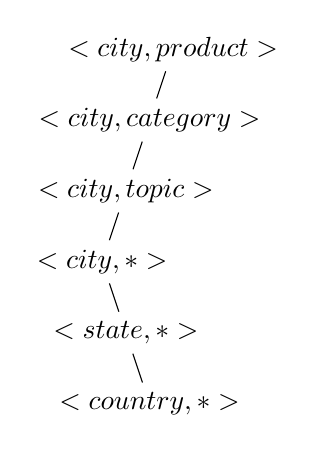
\begin{tikzpicture}[scale=.3]
  \node (co) at (0,-6) {$<country, *>$};
  \node (st) at (-1,-3) {$<state, *>$};
  \node (ci) at (-2,0) {$<city, *>$};
  \node (cito) at (-1,3) {$<city, topic>$};
  \node (cica) at (0,6) {$<city, category>$};
  \node (cipr) at (1,9) {$<city, product>$};
  \draw (co) -- (st) -- (ci) -- (cito) -- (cica) -- (cipr);
\end{tikzpicture}
}
\subfigure[Batch2]{
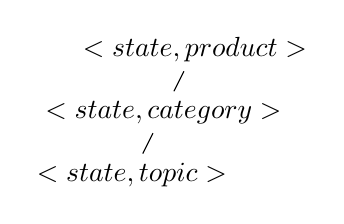
\begin{tikzpicture}[scale=.4]
  \node (stpr) at (0,-2) {$<state, topic>$};
  \node (stca) at (1,0) {$<state, category>$};
  \node (stto) at (2,2) {$<state, product>$};
  \draw (stpr) -- (stca) -- (stto) ;
\end{tikzpicture}
}

\subfigure[Batch3]{
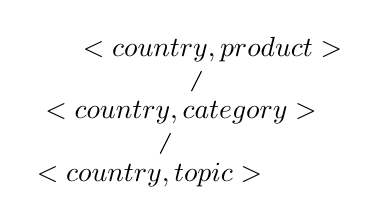
\begin{tikzpicture}[scale=.4]
  \node (stpr) at (0,-2) {$<country, topic>$};
  \node (stca) at (1,0) {$<country, category>$};
  \node (stto) at (2,2) {$<country, product>$};
  \draw (stpr) -- (stca) -- (stto) ;
\end{tikzpicture}
}
\subfigure[Batch4]{
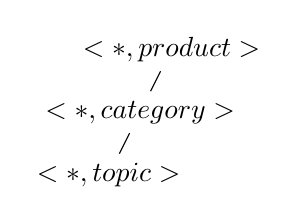
\begin{tikzpicture}[scale=.4]
  \node (stpr) at (0,-2) {$<*, topic>$};
  \node (stca) at (1,0) {$<*, category>$};
  \node (stto) at (2,2) {$<*, product>$};
  \draw (stpr) -- (stca) -- (stto) ;
\end{tikzpicture}
}
\caption{Batching plan}
\label{fig:batch}
\end{figure}

\subsubsection{Postprocess}
The materializate phase ensures that the operation in this phase will be algebraic. We can simply merge the measures of each partial group by adding them together.

\section{Implementation}

We implement the algorithms with Hadoop streaming and Python 2. No third-party package is used in our implementation.

\subsection{Estimate}

First we compute $\rho=\frac{1}{m}\ln(np)$. In the mapper, for each sampled tuple, we output the values in the shortest region for each batch and the uid. Then Hadoop will sort the key i.e. the values in the shortest regions for us. In the reducer, we divide the KVList evenly into $p$ partitions, and output the $p - 1$ boundaries. To preserve consistency, the number of reducer should be 1. This phase is illustrated in Algorithm~\ref{alg:estimate}.

\begin{algorithm}[h]
\centering
\caption{TSCube Estimate}
\label{alg:estimate}
  \begin{algorithmic}[1]
    \Function{Estimate-Map}{data}
      \For{each tuple e in the data}
      	\State Generate a random real number $q$, $q \in [q,p]$
      	\If{$q \leq p$}
      		\For{each Batch B in C}
      			\State k = B(e) \Comment{B(e) returns the values in the shortest region of B}
      			\State \textsc{emit} k $\Rightarrow$ e.uid
      		\EndFor
      	\EndIf
      \EndFor
    \EndFunction
\\
    \Function{Estimate-Reduce}{KVList}
      \State Divide the KVList evenly into p partitions
      \State Extract and emit p − 1 boundaries
    \EndFunction
  \end{algorithmic}
\end{algorithm}


\subsection{Materialize}

\paragraph{}
This phase is illustrated in Algorithm~\ref{alg:materialize}. In the mapper, we determine the partition that a tuple falls in for each batch by the values of the shortest region in the batch and the uid in this tuple. Thus we can globally sort each partition by batch and uid, and make sure that tuples with the same uid in the same batch will go to the same partition. After mapping, we instruct Hadoop to partition the output of mappers by the computed partition id, and sort within each partition by the values of the shortest and longest region to aid cubing in the reducers. 

\begin{algorithm}[h]
\centering
\caption{TSCube Materialize}
\label{alg:materialize}
  \begin{algorithmic}[1]
    \Function{Materialize-Map}{data}
      \For{each tuple e in the data}
      		\For{each Batch B in C}
      			\State k = B(e) + e.uid
      			\State obtain the partition $p_{k}$ that $k$ falls in
      			\State \textsc{emit} k $\Rightarrow$ e to partition $p_{k}$
      		\EndFor
      \EndFor
    \EndFunction
\\
    \Function{Materialize-Reduce}{KVList}
      \State Cube the KVList
    \EndFunction
  \end{algorithmic}
\end{algorithm}

To obtain the partition for each tuple in each batch, we put the results of the first phase into the Hadoop Distributed Cache to avoid extra network I/O. In the mapper, we simply open the cached partition file and use binary search to find the desired partition.

\begin{table}[h]
\centering
\begin{tabular}{l l l l l l}
country & state & city & topic & category & product \\
\hline
1 & 2 & 10 & 1 & 20 & 5 \\
1 & 2 & 13 & 1 & 20 & 5 \\
1 & 2 & 14 & 1 & 20 & 5

\end{tabular}
\caption{In this example, the topics of the records don't change while the city has changed, so the uids in the $Set_{topic=1}$ will all be merged into the $Set_{city=10}$, resulting in wrong measures.}
\label{table:interrupt}
\end{table}

During the implementation, we discover that in batches where there are two hierarchies involved, the field in the first hierarchy would disturb the cubing process of the second one (illustrated in Table~\ref{table:interrupt}). Therefore, we decide to take an approach more simliar to the BUC algorithm mentioned in \cite{beyer1999bottom} than the top-down cubing algorithm discussed in \cite{agarwal1996computation} and \cite{zhao1997array}. Instead of scanning the fields from the top, updating the previous set and output the measures of current field on changes, we scan the fields from the bottom, updating the sets as soon as a new tuple is scanned, and output the measures of following fields on changes. 
\\
This approach would not cost more memory than the original top-down cubing algorithm, since th number and sizes of the sets we need to maintain will not change greatly. The most significant change lies in the number of insertion into these sets. The pseudocode of this algorithm is explained in Algorithm~\ref{alg:cubeal}.

\begin{algorithm}[H]
\centering
\caption{The cubing algorithm}
\label{alg:cubeal}
\begin{algorithmic}[1]  
\For{each K-V pair}
	\State $B \Leftarrow$ the batch this K-V pair belongs to
	\State $dim \Leftarrow$ The starting dimension of B
	\State $numDims \Leftarrow$ The total number of dimensions of B
	\For{$i=dim$; $i<numDims$; $i++$ }
		\If{The field in $i$ changes}
			\State Output the measure of this and each subsequent dimensions
			\State Update the sets of this and each subsequent dimensions
			\State \textbf{break}
		\Else
			\State Add the uid into $Set[i]$
		\EndIf
	\EndFor
\EndFor   
\end{algorithmic}  
\end{algorithm}

\subsection{Postprocess}

The post processing is relatively simple. Since the materialization ensures that this phase will be algebraic, all we need to do is add the measures of each partial cube together, as illustrated in Algorithm~\ref{alg:post}.

\begin{algorithm}[H]
\centering
\caption{TSCube Postprocess}
\label{alg:post}
  \begin{algorithmic}[1]
    \Function{Postprocess-Map}{data}
      \State Pipe the data through
    \EndFunction
\\
    \Function{Postprocess-Reduce}{group, \{$v_{1}, v_{2}, ...$\}}
      \State $v_{final} = \sum{v_{i}}$
      \State \textsc{emit} group $\Rightarrow v_{final}$
    \EndFunction
  \end{algorithmic}
\end{algorithm}

\section{Experiments}

\subsection{Environment settings}

\paragraph{}
We perform the experiment on a cluster made up of our laptops. There are 4 nodes in total, 3 of them are slaves, each of them runs Hadoop-1.0.4 and Python 2.7+. The hardware environment is listed in Table~\ref{table:env}. We use the standard CPython intepreter to execute the programs, though presumably other optimized implementation (e.g. PyPy) should accelerate the execution.

\begin{table}[h]
\centering
\begin{tabular}{l l l l l}
Role & OS & Memory & CPU & Disk \\
\hline
Master & Ubuntu 12.04 & 3848M & Intel i7-3517U & 256GB \\
Slave & Ubuntu 13.04  & 7882M & Intel i7-3610QM & 500GB \\
Slave & Ubuntu 13.04 & 1978M & Intel Pentium B950 & 500GB \\
Slave & Ubuntu 13.04 & 3547M & Intel i3-2330MB & 500GB
\end{tabular}

\caption{Hardware environment}
\label{table:env}
\end{table}

\subsection{Experimental results on the cluster}

The experimental results is shown in Figure~\ref{fig:performance}. The Naive Cube outperforms TSCube for small datasets due to the extremely low overhead costs, as is consistent with the description in \cite{nandi2012data}. But when the size of the dataset goes up, TSCube starts to perform better than the Naive approach, while Naive Cube just fails when the size of the dataset reach a certain point due to the burden of intermediate data and size of large groups.

\begin{figure}[H]
\centering
\begin{tikzpicture}
\begin{loglogaxis}[
title={Performance of Naive cube and TSCube},
xlabel={Data Size},
ylabel={Time(s)},
legend pos=outer north east
]
\addplot table[x=size,y=naive] {naive.dat};\addlegendentry{Naive}
\addplot table[x=size,y=tscube] {tscube.dat};\addlegendentry{TSCube}
\end{loglogaxis}
\end{tikzpicture}

\caption{Performance of Naive cube and TSCube}
\label{fig:performance}
\end{figure}

\bibliography{tscube}

\end{document}